Den strategi som vann flest poäng var Tit for tat, som samlade ihop lite över 30 000 poäng. Figur \ref{points} nedan beskriver hur många poäng varje strategi samlade ihop.

\begin{figure}[htb]
	\begin{center}
	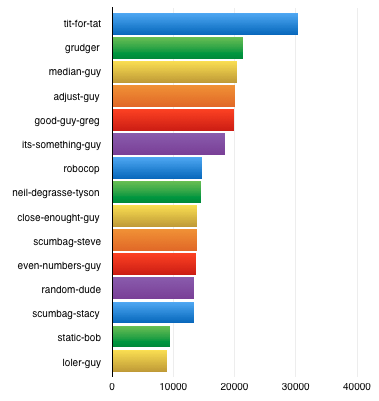
\includegraphics[scale=0.75, angle=0]{bilder/points.png}
	\caption{Totalt antal poäng efter 1000 omgångar.}
	\label{points}
	\end{center}
\end{figure}

Gemensamt för de tre bästa strategierna är att de tar hänsyn till motståndarens historik. Gemensamt är också att Tit for tat och Grudger startar alltid på 10 och Median guy startar på ett slumpmässigt tal, vilket kan vara 10. 

\newpage

Den strategi som vann flest gånger var tit-for-tat, alltså vann tit-for-tat både flest vinster och flest poäng. Figur 2 nedan beskriver hur många vinster respektive strategi tog. Topp tre i figur \ref{points} och figur \ref{wins} består av samma strategier. Strategierna Tit for tat, Grudger och Median guy är med andra ord både pålitliga och effektiva. 

\begin{figure}[htb]
	\begin{center}
	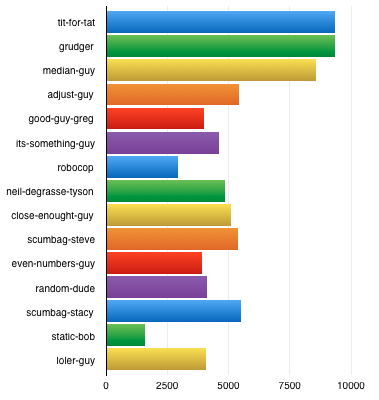
\includegraphics[scale=0.75, angle=0]{bilder/wins.png}
	\caption{Totalt antal vinster efter 1000 omgångar.}
	\label{wins}
	\end{center}
\end{figure}

<<<<<<< HEAD
=======
De båda figurerna visar tillsammans att de strategier som vinner flest gånger också är de som får mest poäng av alla. 

\begin{figure}[htb]
	\begin{center}
	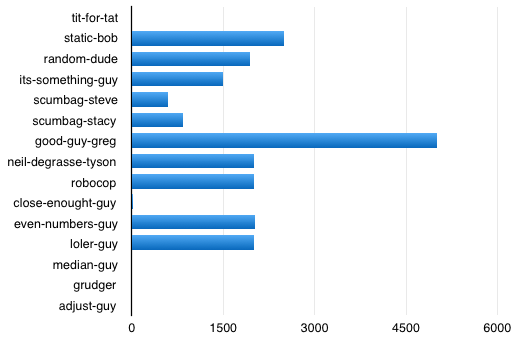
\includegraphics[scale=0.75, angle=0]{bilder/adjust-guy.png}
	\caption{Detta är bildtexten}
	\label{adjust-guy}
	\end{center}
\end{figure}

\begin{figure}[htb]
	\begin{center}
	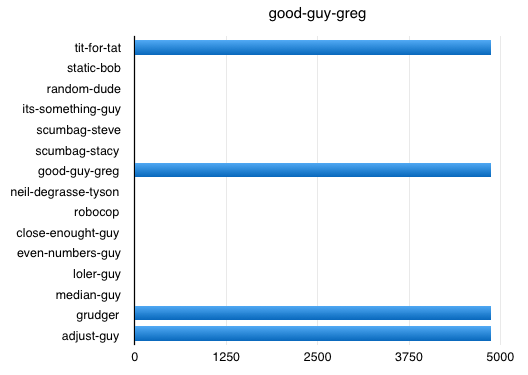
\includegraphics[scale=0.75, angle=0]{bilder/good-guy-greg.png}
	\caption{Detta är bildtexten}
	\label{good-guy-greg}
	\end{center}
\end{figure}

\begin{figure}[htb]
	\begin{center}
	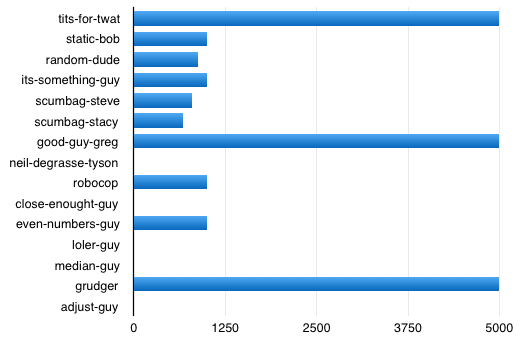
\includegraphics[scale=0.75, angle=0]{bilder/grudger.png}
	\caption{Detta är bildtexten}
	\label{grudger}
	\end{center}
\end{figure}

\begin{figure}[htb]
	\begin{center}
	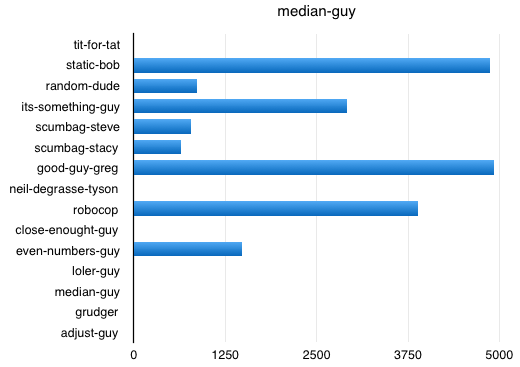
\includegraphics[scale=0.75, angle=0]{bilder/median-guy.png}
	\caption{Detta är bildtexten}
	\label{median-guy}
	\end{center}
\end{figure}

\begin{figure}[htb]
	\begin{center}
	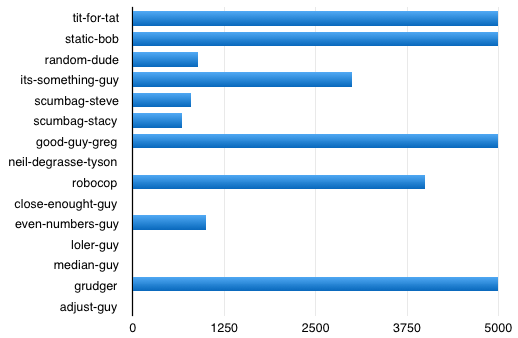
\includegraphics[scale=0.75, angle=0]{bilder/tit-for-tat.png}
	\caption{Detta är bildtexten}
	\label{tit-for-tat}
	\end{center}
\end{figure}
>>>>>>> FETCH_HEAD
